	\begin{enumerate}
	\item Цель:
		\begin{itemize}
			\item Найти и поставить более прочные оси, способные выдерживать подобную нагрузку
			\item Усилить механизм передвижения подъемника
			\item Сделать конструкцию подъемника более стабильной
		\end{itemize}
	\item Реализация: 
		\begin{itemize}
			\item Программа была написана для второго оператора, управление высотой подъема происходит через джойстик, в будущем будет установлен резервуар для временного хранения шариков, который будет открываться/закрываться при помощи сервопривода по команде оператора.
			\item Устойчивость подъемника была увеличена путем установки второй оси, соединяющий две стороны подъемника. На самом верху конструкции были установлены еще две выдвижные рейки, повышающие стабильность конструкции и позволяющие с большей легкостью установить резервуар.(Рисунки 16, 17)
			\item Исправить слишком сильное выгибание оси под нагрузкой удалось путем жесткого закрепления оси на специальных креплениях, установленных на конструкции робота.(Рисунок 18)
			\begin{minipage}{0.3\linewidth}
			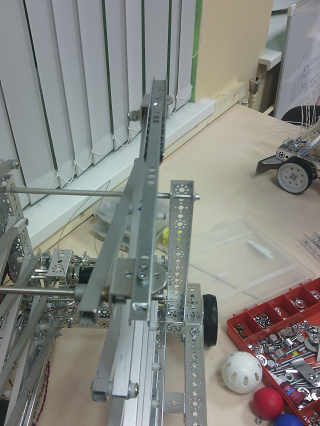
\includegraphics[width=45mm,height=45mm]{Days/10.11.14/11_1_robot}\\ Рисунок 16
			\end{minipage}
			\begin{minipage}{0.3\linewidth}
			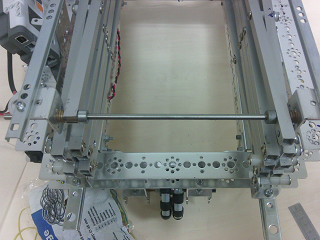
\includegraphics[width=45mm,height=45mm]{Days/10.11.14/11_2_robot}\\ Рисунок 17
			\end{minipage}
			\begin{minipage}{0.3\linewidth}
			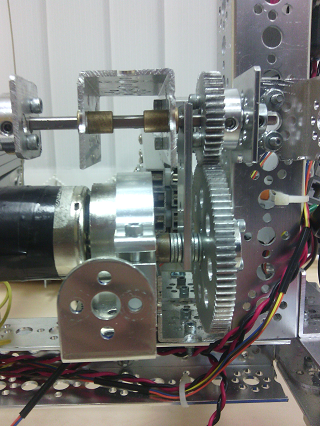
\includegraphics[width=45mm,height=45mm]{Days/10.11.14/11_4_robot}\\ Рисунок 18
			\end{minipage}
		\end{itemize}
		\newpage
		\item Идеи и планы:
			\begin{itemize}
				\item Доделать резервуар и установить на него сервопривод
				\item Попытаться сделать что-либо для возвращения подъемника в изначальное - сложенное - состояние, так как под собственным весом он этого сделать не может.
			\end{itemize}
\end{enumerate}
\fillpage
